The system has been used to identify certain patterns in different types of multivariate time-series. In this section, we highlight several examples - the first from synthetically generated data followed by two real world datasets. Finally we describe some other examples of the use of system.

\subsection{Prediction Evaluation}

This first experiment is intended to test the validity of our model. The model was constructed on simulated data of 
an electric motor and is shown in Figure \ref{fig:example-motor}. 
\begin{figure*}[]
  	\centering
  	\begin{subfigure}{.48\textwidth}
	  	\centering
	  	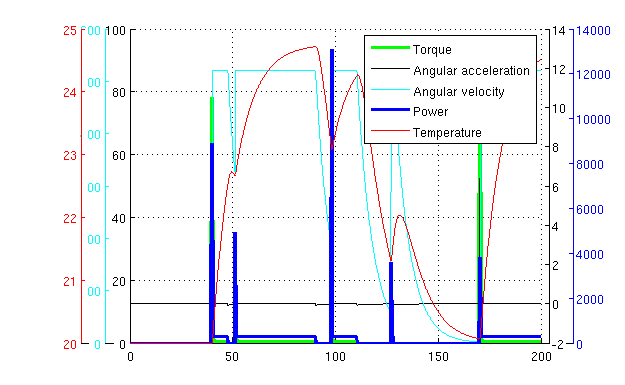
\includegraphics[width=\columnwidth]{simulation-processed}
  		\caption{\label{fig:simulation-chart}\lstopar{TODO}}
	\end{subfigure}
  	\begin{subfigure}{.48\textwidth}
	  	\centering
	  	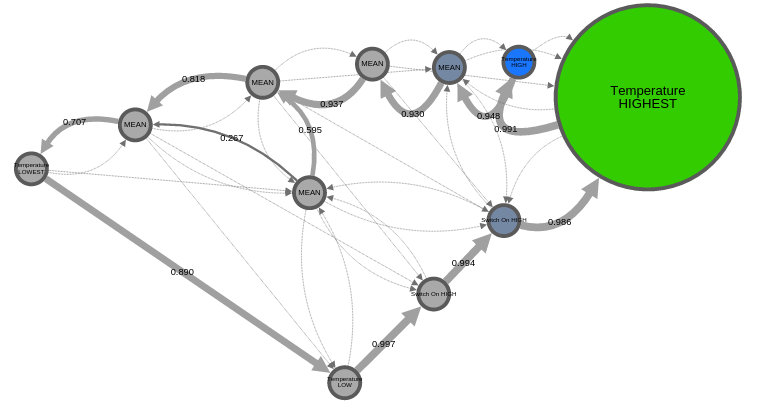
\includegraphics[width=\columnwidth]{model-motor-simulated}
  		\caption{\label{fig:simulation-model}\lstopar{TODO}}
	\end{subfigure}
  	\caption{\lstopar{TODO}}
  	\label{fig:example-motor}
\end{figure*}
The simulation starts in the leftmost state of Figure~\ref{fig:simulation-model} with the motor in a stationary state
and the power switch turned off. Then \lstopar{an invisible user} randomly, sampled from an exponential distribution,
toggles the ``on" switch. Once the switch is on, as the rotation increases, the model starts moving in the counter clockwise
direction towards the large green state on the right. This state represents the \lstopar{equilibrium} when the temperature
gained through friction equals the temperature lost to the ambient and the \lstopar{signals} become \lstopar{stationary}.
Once the power switch is toggled again, the rotation slowly halts due to friction and the process goes from right to
left in the counter clockwise direction.

To conduct the experiment we generated two dataset: a training set and a test set. Both datasets
contained $200k$ observations. We built a StreamStory model with 20 lowest-level states on the training set using two attributes:
angular velocity and temperature. The training dataset was then replayed through the model and the finest scale states were stored. We then used
the stored states to calculate the transition probabilities and compared them to the models' jump chain $\Pi$. Since a lot of these probabilities were zero, we decided to use only the probabilities that
are non-zero either in the jump chain or in the probabilities calculated from the history. We then
computed the mean absolute error of the non-zero probabilities which resulted in $MAE=0.05$ or $5\%$.

In another experiment we tested the models predictive power. Two StreamStory models were built: (a) one 
model using the same attributes as in the first experiment, while in the second model (b), we used
the logical switch signal to model state transitions. The models were trained on the same dataset
as in the first experiment. Before the process jumped, we extracted the next state probabilities
and used the state with the highest probability as the predicted next state. We then computed
the prediction accuracy as the ratio between the number of correct predictions and the total number
of jumps (total number of predictions). In this experiment model (a) scored $0.845$ while model
(b) scored $0.904$.


\subsection{Weather Data}
\label{sec:experiments-weather}

The example below shows our model generated on monthly rainfall and temperature data
collected over the course of 20 years between 1920 and 1940 in Nottingham, England.

\begin{figure}[h!]
	\centering
	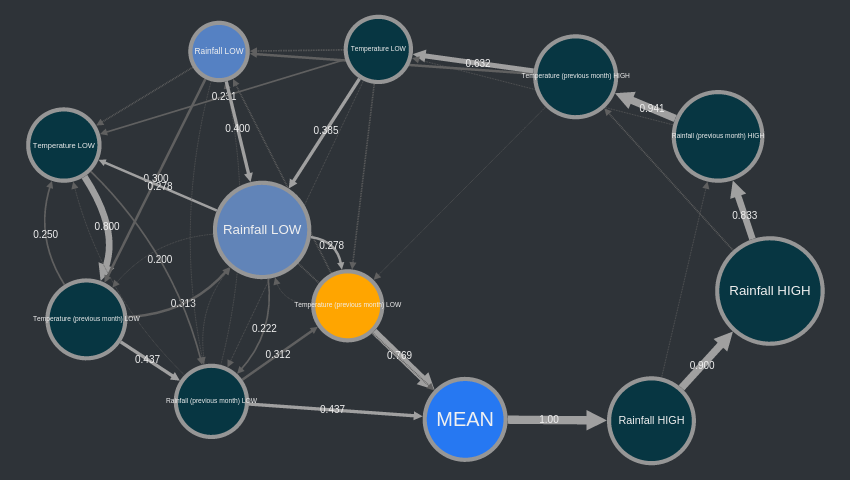
\includegraphics[width=\columnwidth]{example-weather}
	\caption{Qualitative representation of temperature and rainfall data collected over the course of 20 years. The yearly timeline flows in the clockwise direction with the right-most state representing the summer, the bottom states representing autumn, the left-most states representing winter and the top states representing spring.}
	\label{fig:example-weather}
\end{figure}

The model was generated using the raw rainfall and temperature data, lifted into a four dimensional space.
\lstopar{Lifting was done as suggested in Section \ref{sec:preliminaries} by appending the previous sample to the current sample, effectively adding two new dimensions}.

The states on the right hand side represent the 
summer states, while the states on the left represent winter states. The yearly timeline flows in the clockwise direction with the spring states residing on the bottom of the figure and the autumn
states on the top.

Interestingly, in this dataset, the rainfall and temperature are very correlated and the auto labeling feature
choose high rainfall as the most significant feature of the summer states. This correlation can be seen
from the attribute histogram shown in Figure \ref{fig:histograms-summer}.

Using our model, we can clearly see how the summer and winter dynamics differ. While the summer states seem to be quite deterministic, with a high probability of jumping into the next state in the clockwise direction, the transition probabilities in the winter states are much more uniform, suggesting larger fluctuations in the weather during the winter.

\begin{figure}[h!]
	\centering
	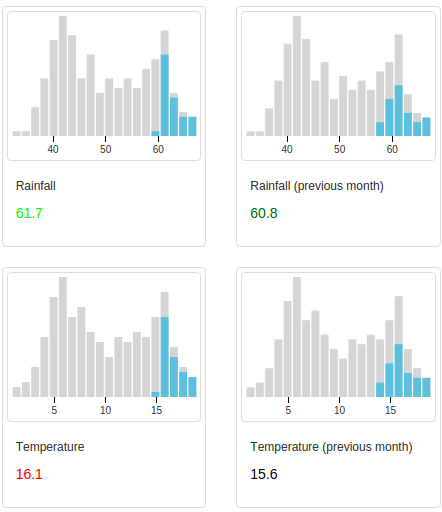
\includegraphics[width=0.5\columnwidth]{histograms-summer}
	\caption{\lstopar{TODO caption}}
	\label{fig:histograms-summer}
\end{figure}

\subsection{GPS Data \lstopar{[TODO change description to fit the data]}}

The second example was created using raw GPS coordinates collected using a smartphone between years 2012 and 2015.
The data represents the everyday movement of a European computer science researcher. Figure \ref{fig:example-geo}
shows our qualitative representation of this data on a high level with 8 states.

\begin{figure}[h!]
	\centering
	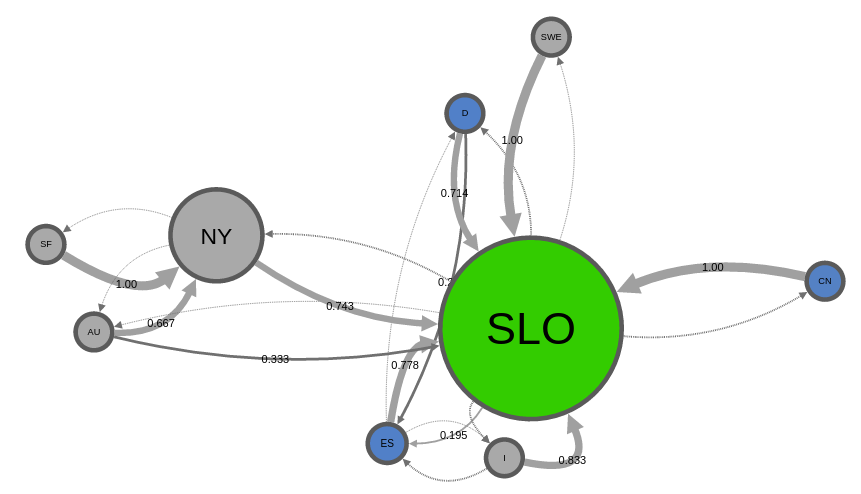
\includegraphics[width=\columnwidth]{geo-states}
	\caption{\lstopar{TODO caption}}
	\label{fig:example-geo}
\end{figure}

From the figure, we can see that the system was able to identify the most typical locations of this persons
movements.

They spent most of the time in south-central Europe including the central green state and the bottom-most state. The small state on the right represents India, where they went for vacation last year. On the European continent, the system
also identified Germany and Sweden where the person frequently attends meetings or stays for a short while
during a connecting flight. The states on the left represent the USA with the largest state representing New
York city where the person spent the 2014 summer and the smaller states representing San Francisco and Austin,
Texas.

\subsection{Traffic Data}

Our next example, shown in Figure \ref{fig:example-traffic}, shows a representation of a traffic counter positioned on the highway ring around Ljubljana, Slovenia.
\lstopar{In this example, we lifted the counter into a three dimensional space, by also including the number of
cars three hours and one day before.}
\begin{figure}[h!]
	\centering
	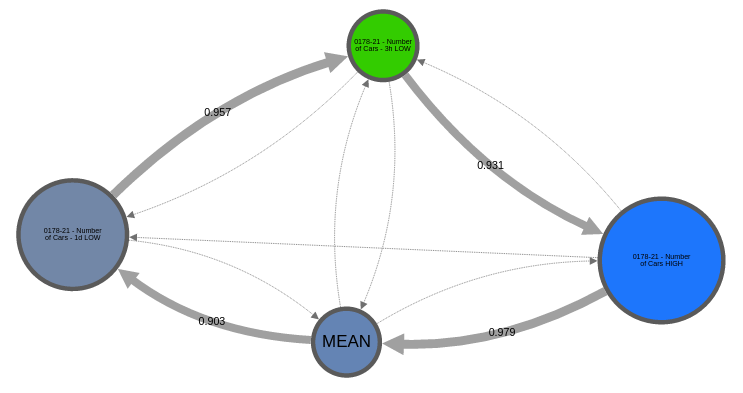
\includegraphics[width=\columnwidth]{example-traffic}
	\caption{\lstopar{TODO caption}}
	\label{fig:example-traffic}
\end{figure}
On a high level, our system was able to identify what we believe is the typical daily cycle on the highway ring.
The state on the left hand side represents a night state, when the traffic traffic is the lowest. This state
lasts from 10 PM to 5 AM when most people are asleep and not much is happening on the road. Then, with a high 
probability, the system jumps into the topmost state with an above average traffic count which lasts from 6 AM
to roughly 9 AM. The next state is the midday state on the right with the highest traffic count lasting from 9 AM
to 7 PM. This is exactly the time when the traffic is very dense and most congestions occur. The next transition
is to the bottommost ``evening" state with an average traffic count between 300 and 1000 cars per \lstopar{hour},
lasting from 8 PM to approximately 10 PM. 

\primoz{
\begin{itemize}
\item Here we also need some examples of where its not useful -  a few different scales and we need references on the data. These can be deliverables. 
\item Also we should show how much information we lose over different scales.
\end{itemize}}

\subsection{Domain Experts}
In the above examples, the discovered states could be interpreted by non-experts. We have also tested the system in more specialized settings. One example the system was tested on measurements from an oil drilling platform\footnote{Unfortunately, at the time of submission, we were not cleared to share the results of the analysis, including an evaluation on useability.}. In this data, natural recurrent behaviour was detected.  The model also detected an ``event,'' where certain equipment failed and drilling needed to be halted.  

%A second example is based on a manufacturing plant. In this case, we cannot 

